%tRNA document
%\documentclass[pdftex, 12pt, twocolumn]{article}
\documentclass[pdftex, 12pt]{article}
\usepackage{enumerate}
\usepackage{amsmath, amstext, amsfonts, amssymb}
\usepackage{setspace}
\usepackage[pdftex]{graphicx}
\usepackage[left=2.54cm,bottom=2.54cm,top=2.54cm,right=2.54cm]{geometry}
\singlespacing
\begin{document}
\author{Prerana Pradhan}
\title {A review on tRNA\\
\bigskip
\normalsize{End of Semester Report at Wilma K. Olson's Lab.}}
\maketitle
\section{Introduction} 
Transfer ribonucleic acid, or tRNA, is an RNA molecule that transfers amino acids to form a polypeptide chain at the ribosomal site of protein synthesis during translation. It has a 3-base region (e.g. see Figure one A36, A35, g34) called an anticodon, which can base pair to a corresponding codon region on messenger ribonucliec acid (mRNA) on mRNA. Therefore, the role of tRNA is to bond with amino acids and form aminoacyl tRNAs. Aminoacul tRNAs are then 'transfered' to the ribosomes in a cell, where proteins are assembled according to the genetic code of  mRNA, which has been transcribed from DNA into mRNA. tRNAs are used in phylogenetic studies of evolution and medical research. For example, tRNA plays a big role in reverse transcriptase in  human immunodeficiency virus, or HIV-1. In the virus, there is an enzyme called reverse transcriptase, which is an enzyme that produces double stranded DNA copies of the single stranded RNA genome in the HIV-1 virus. In particular, the production of double stranded DNA is primed by the host cell lysine-tRNA.  

\subsection{History of tRNA} 
In an unpublished letter to the RNA tie club in early 1955, the idea  of tRNA was introduced by Francis Crick \cite{crick1958}. The structure was not researched significantly til the 1960s, when it was scrutinized by Alex Rich and Don Caspar from Boston, Massachusetts. Others who researched tRNA include the Jacques Fresco group at Princetion University, and a group from King's  College London. Robert W. Holley first published the primary structure in 1965. A group headed by Alexander Rich and Aaron Klug analyzed the secondary and tertiary structures, which they derived from X-ray crystallography in 1974.

\subsection{Structure of tRNA} 
tRNA can be describe at three structural levels, which are the primary, seconday, and tertiary structures. The primary structure corresponds to the nucleotide sequence. The secondary structure is usually seen in a cloverleaf type, while the tertiary structure is L shaped, which helps the tRNA  fit into the ribosome. In tRNA, the 5'terminal is a phosphate group. The acceptor stem is made by the base pairing of the 5'-terminal nucleotide with the 3'-terminal nucleotide. The D arm is a 5  base pair stem that ends in a loop which contains dihydrouridine. Similarly, the anticodon arm is a 5 base pairstem with a loop that contains the actual anticodon. The T arm is also a five base pair stem; it contains pseudouridine. Any bases that can be modified, usually by methylation, are located outside the anticodon. The first anticodon base can be modified into the following: inosine, which is derived from adenine, or pseudouridine,which is derived from uracil. This figure made using 522 (RNAview) shows convention for Watson-Crick base pairing as well as non-canonical base pairing. 
\begin{figure}[ht]
  \begin{minipage}[b]{0.5\linewidth}
    \centering
    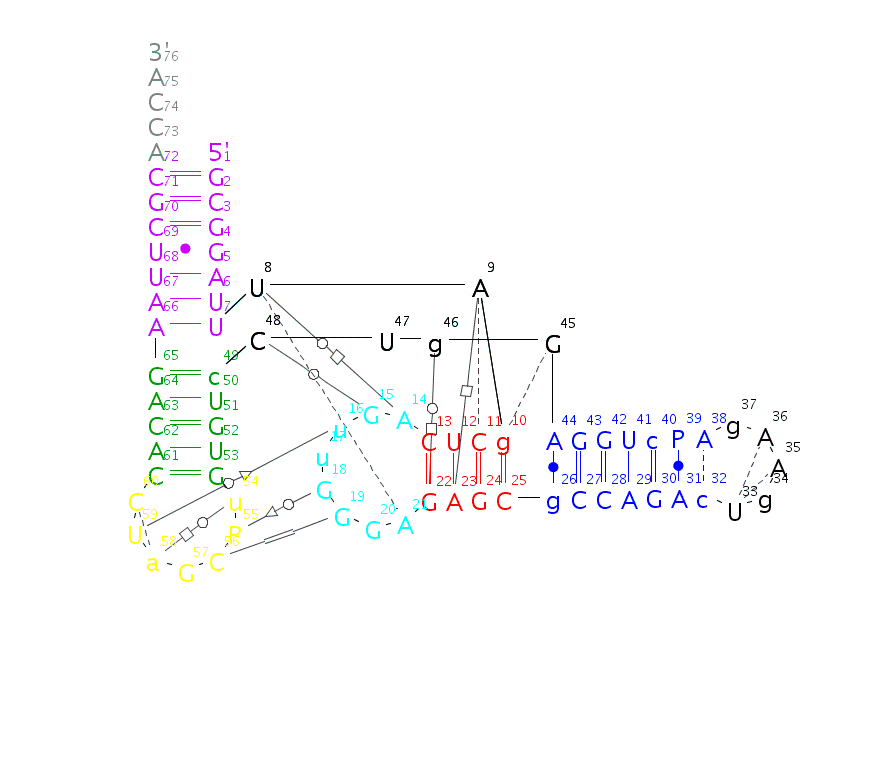
\includegraphics[scale=.35]{secstrtRNA.png}
    \caption{2-D tRNA}
    \label{fig:figure1}
   \end{minipage}
   \hspace{0.5cm}
   \begin{minipage}[b]{0.5\linewidth}
     \centering
     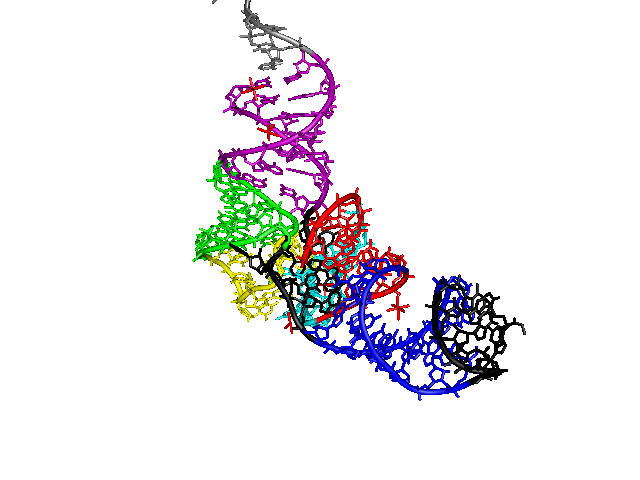
\includegraphics[scale=.35]{secstrtRNA_2.png}
     \caption{3-D tRNA}
     \label{fig:figure2}
    \end{minipage}
\end{figure} Figures  1 and 2  present tRNA structure  in 2-dimesional
and 3-dimensional  form. The tRNA figures are  dissected and sectioned
off according to colors. The grey represents the CCA tail, the

\subsection{Definition:  Anticodon} Anticodons  are made  up  of three
nucleotides  each;  these  nucleotides  correspond to  the  codons  on
mRNA. The  tRNA contains  specific sequences that  match up to  one or
more codons  for an  amino acid.  For example, a  codon for  lysine is
AAA. Consequently, and anticodon for lysine on tRNA would be UUU. When
anticodons pair with  more than one codon, it is  known as wobble base
pairing. It is common for an amino acid to occup four possibilities in
the genetic code.  This can be seen in a case  like glycine, which can
be coded for by GGU, GGC, GGA, and GGG.

\subsection{Definition:  Aminoacylation} Aminoacylation is  defined as
'the process of adding an  aminoacyl group to a compound.'This process
makes tRNA that  have their CCA 3' ends covalently  linked to an amino
acid. Every tRNA is charged with  an amino acid through the work of an
aminoacyl  tRNA  synthetase.  Usually,  there is  one  aminoacyl  tRNA
synthases  for  each amino  acid.  In  PDB,  there are  126  aminoacyl
synthetase structures.

\subsection{Repositories}   There  are   over   2000  tRNA   sequences
available. Any  protein data bank  will have information on  tRNA. The
Zurich Open  Repository and Archive,  the YRC Public  Data Repository,
and the  well known PDB.  A database that  is specific to tRNA  is the
aminoacyl-tRNA   synthetases   database.  Aminoacyl-tRNA   synthetases
(AARSs)   are  the   key  components   of  the   protein  biosynthesis
machinery.  They  are  responsible  for maintaining  the  fidelity  of
transfer of genetic information from DNA into protein. The database is
a  compilation   of  amino   acid  sequences  of   all  aminoacyl-tRNA
synthetases known to  date; it contains 422 primary  structures of the
AARSs available as separate entries or alignments of related proteins.
Another useful tRNA repository  is probably the genomic tRNA database,
which contains  tRNA whose structures  have been analyzed  through the
program tRNA  scan-SE. As mentioned before, tRNAs  consist of primary,
secondary, and  tertiary structures.  These structures can  be further
research in the genomic tRNA  database as well.  The Protein Data Bank
has  41915 tRNA  structures evaluated  by x-ray,  and  7115 structures
evaluated by NMR.

\subsection{Question and Answer}
While researching tRNA, some questions emerged, which we present here. 
\begin{enumerate}
\item
How many tRNA crystal structures are there in the PDB?

The protein data bank lists that there are currently 678 tRNA crystal structures available. 
\item
Which is the main database for tRNA sequences?

The Genomic tRNA Database, or GtRNAdb details many tRNA identifications with complete or nearly complete genomes. Another data base, supervised by Bayreuth University in Germany, consists of a compilation of tRNA sequences and sequences of tRNA genes. 
\item
What are conserved regions? Which are the most conserved bases in tRNA?

Protein homologs can be defined as amino acid sequences with a common evolutionary ancestor. However, sequence changing process such as substitutions, insertions, and deletions cause homologs to drift or branch off from each other over time. Conservation profiles serve as measures of the common patterns that still persist.\cite{Vries2008} Thus, conserved regions are those sequences that are consistent over eveolutionary time. Some common residues are those at the 32, 38, and 37 positions. Other highly conserved groups are defined by the residue at the first wobble anticodon position.\cite{saks2007}  
\item
What is Crick's Wobble hypothesis?

In 1966, Francis Crick proposed that while the interaction between the codon in the mRNA and the anticodon in the tRNA need to be exact in two of three nucleotide positions, this is not necessary in the third position. He thus stated that non-standard base-pairing might occur between the nucleotide base in the 5' position of the anticodon and the 3' position of the codon.\cite{crick1966}
\item
What are cognate, near-cognate, and non-cognate tRNAs?

Cognate tRNAs fully and properly decode genetic information in mRNA. Near-cognate tRNAs correspond to tRNAs that somewhat decode the genetic information, and non-cognate tRNAs do not decode at all. 

\end{enumerate}

 

%\subsection{References}
\bibliographystyle{plain}
\bibliography{biblio}	



\end{document}
